\chapter{Project realization}
\section{Introduction}
This chapter covers the implementation, testing and the deployment processes of
the Benchmarks dashboard project. To deal wit each of these processes, we will
introduce the technologies used and describe the way we used them. In
addition, we will presente the project planning.
\pagebreak

\section{Used technologies}
\subsection{Programming languages}
\subsubsection{Python}
Python is an interpreted, interactive, object-oriented programming language. It
incorporates modules, exceptions, dynamic typing, very high level dynamic data
types, and classes. Python combines remarkable power with very clear syntax. It
has interfaces to many system calls and libraries, as well as to various window
systems, and is extensible in C or C++. It is also usable as an extension
language for applications that need a programmable interface. Finally, Python is
portable: it runs on many Unix variants, on the Mac, and on PCs under MS-DOS,
Windows, Windows NT, and OS/2.

Python is a high-level general-purpose programming language that can be applied
to many different classes of problems. The language comes with a large standard
library that covers areas such as string processing (regular expressions,
Unicode, calculating differences between files), Internet protocols (HTTP, FTP,
SMTP, XML-RPC, POP, IMAP, CGI programming), software engineering (unit testing,
logging, profiling, parsing Python code), and operating system interfaces
(system calls, filesystems, TCP/IP sockets). Look at the table of contents for
The Python Standard Library to get an idea of what’s available. A wide variety
of third-party extensions are also available.
TODO(Add link Python https://docs.python.org/2/faq/general.html)

\subsubsection{Javascript}
JavaScript (shortened to JS) is an interpreted, object-oriented, weakly typed,
programming language with first-class functions most known as scripting language
for Web pages. It was originally implemented so that client-side scripts could
interact with the user, control the browser, communicate asynchronously and
alter the web page content that was displayed, and now it has evaluated to
involve game  development and applications creation. JavaScript's main purpose
was the creation and embedding of scripts in the HTML client side in order to
guarantee more interactivity with the user. It was created to offer dynamic
tasks such as the transformation of the page elements, visual effects and
immediate reactions to the user actions. But now JS for server-side web is
gaining popularity with the appearance of JavaScript frameworks for that
purpose. 
JavaScript was a purely interpreted language. This means that scripts execute
without preliminary compilation (without conversion of the script text into
machine code). The user's browser interprets the script, that is, analyzes and
immediately executes it. In modern implemented, The user's browser interprets
the script, that is, analyzes and immediatley 
TODO(Add link Mozilla developer network, https://developer.mozilla.org/en-us/docs/web/javascript)

\subsection{Frameworks}
\subsubsection{Pyramid}
Pyramid is a fast and low-level Python web framework. It is developed as
part of the Pylons Projects. Even Pyramid isn't famous like Flask and Django, it
minimal, unobtrusive and agnostic design helps in developing more robust and
fast web applications. TODO(Complete) 

\subsubsection{ReactJS}
React is an open-source front end library developed by Facebook. It's used for
handling view layer for web and mobile apps. ReactJS allows us to create large
web applications that use data which can change over time, without reloading the
page, using reusable UI components. Its main goal is to be fast, simple and
scalable. It is currently one of the most popular JavaScript libraries and it
has strong foundation and large community behind it. React components are
typically written in JSX, a JavaScript extension syntax allowing quoting of HTML
and using HTML tag syntax to render subcomponents.

\subsubsection{Grommet}
Grommet is a UX framework for enterprise applications developed by HP, on top of
ReactJS. It was created to align the desing and developer workflow into one
seamless experience. The Grommet components library is designed to be perfect
complement to the design system. With little setup, developer will be able to
create a Grommet application from scratch in minutes and take the pain out of
translating desing files into unning application code.

\section{Tools and services}
\subsection{AWS}
Amazon Web Services (AWS) is a subsidiary of Amazon.com that provides on-demand
cloud computing platforms. These services operate from many global geographical
regions including 6 in North America. They include Amazon Elastic Compute
Cloud, also known as "EC2", and Amazon Simple Storage Service, also known as
"S3". As of 2016, AWS has more than 70 services, spanning a wide range,
including compute, storage, networking, database, analytics, application
services, deployment, management, mobile, developer tools and tools for the
Internet of Things. Amazon markets AWS as a service to provide large computing
capacity quicker and cheaper than a client company building an actual physical
server farm.

\subsection{Nix}

Nix is a purely functional package manager. This means that it treats packages
like values in purely functional programming languages such as Haskell — they
are built by functions that don’t have side-effects, and they never change after
they have been built. Nix stores packages in the Nix store, usually the
directory /nix/store, where each package has its own unique subdirectory such as

\colorbox{Gray}{\lstinline{nix/store/b6gvzjyb2pg0kjfwrjmg1vfhh54ad73z-firefox-33.1/}}

Where \colorbox{Gray}{\lstinline{b6gvzjyb2pg0...}} is a unique identifier for the package that captures all its
dependencies (it’s a cryptographic hash of the package’s build dependency
graph). This enables many powerful features.

Nix was created by Eelco Dolstra as he's PHD. Eelco is, along with other main
contributors to the Nix ecosystem, a Predictix employment.
\subsubsection{Nix language}
The Nix expression language is a pure, lazy, functional language. Purity means
that operations in the language don't have side-effects (for instance, there is
no variable assignment). Laziness means that arguments to functions are
evaluated only when they are needed. Functional means that functions are
“normal” values that can be passed around and manipulated in interesting ways.
The language is not a full-featured, general purpose language. Its main job is
to describe packages, compositions of packages, and the variability within
packages.

\subsubsection{NixOS}
Nixos is Linux distribution built on top of the Nix package manager. It
uses the Nix language for declarative configuration which allows realiable
system upgrades.
Although NixOS started as a research project, it is a fully functional and
usable operating system.

\subsubsection{NixOps}
NixOps is a tool for deploying sets of NixOS Linux Machines, either to real
hardware or to virtual machines. It extends NixOS's declarative approach to
system configuration to networks and adds provisioning.

\par
The NixOps Dashboard is a built-in house extension to NixOps and offers the same
content and functionality via a Web UI and a rich RESTful API. Core features
are:

\begin{itemize}
\item User-friendly web-based interface
\item Improved security
\item Scheduled operations (deployments, backups, ...etc)
\item Permanent traceability
\item Clear audit trail
\item Role based access
\end{itemize}

We will be using NixOps Dashboard API to provision servers and deploy the
applications in the cloud in order to benchmark them in a production-like
systems.

\section{Developmnet environment}
\subsection{Devlopment machine characteristics}
Below are the characteristics of the developmnet machine we used during the
project implementation.

\begin{itemize}
  \item{\textbf{Processor}: Intel® Core™ i7-3540M CP}
  \item{\textbf{RAM}: 16 GO DDR3 }
  \item{\textbf{System}: Ubuntu Linux 14.04 LTS}
\end{itemize}


\section{Project management}
This section gives an overview of the project management process of the
Benchmarks Dashboard application. At first, we will start by introducing the
project team and then we will describe the tracking process of the different
implementation tasks.
\subsection{Project team}
The table TODO introduces the project team members and their roles.

\begin{center}
  \begin{tabular}{ | p{3cm}  | p{6cm} |}
    \hline

    Scrum role    & Person          \\ \hline

    Product owner & Oussama Elkaceh \\ \hline
    Scrum Master  & Wassel Msehli   \\ \hline
    Team members  & Chaker Benhamed \\ \hline

    \hline
  \end{tabular}
\end{center}

\subsection{Jira}
Predictix development teams use Jira for managing the projects. Jira is a
commercial software product developed by Atlassian. It is used for bug tracking,
issue tracking and project management. Jira allow prioritizing, assigning,
tracking, reporting and auditing issues. Indeed, it improves productivity by
cutting down on time wasted on tracking issues and coordination. In fact, it
keeps the team on track and allows the project manager to monitor the progress
on projects. Besides, it improves quality be ensuring that all tasks are
recorded down with all details and followed up until accomplishment. Moreover,
Jira is an extensible platform which means that it offers workflow customization
to match more the business process. TODO(Add link Atlassian, jira software
provider, www.atlassian.com.)


\section{Implementation}
\subsection{Achieved work}
This section is a description of the four sprints and the results we achieved at
the end of all of the sprints.
\subsection{Sprint 1}
In the first sprint, our goal is to start by automating the benchmark of one of
Predictix's applications, thus we can understand how to generalize for all other
project and solve issue of consistency. The application we worked on is THD-AP.
We started by installing the application locally understand how to build it,
deploy it and how to benchmark it. After getting acquainted to the benchmark
process. We used Nixops Dashboard to deploy the applicatoin on the cloud and
automate the running of tests via systemd servies.

\subsection{Sprint 2}
In the second sprint, our goal is to model the web application that the users
will use to both start benchmarks and visuilaze the benchmarks runs. We stated
by looking the available frameworks for web development. Finally we developed
the workflow that will run new benchmark.

\subsection{Sprint 3}
In the second sprint, our goal is to model the web application that the users
will use to both start benchmarks and visuilaze the benchmarks runs. We stated
by looking the available frameworks for web development. Finally we developed
the workflow that will run new benchmark.

After we get acquainted to the benchmark process, we started righting defining
the steps in the benchmark pipeline. 
\subsubsection{Deploying}
To be tested in production-like environment, the
application need to be deployed to the cloud. In order to compare between
benchmarks runs the server in which the application will be deployed need to be
consistent across all the runs The user mustn't have any interaction with the
provisioning of the server nor the deployment of the application. 

$\bullet$ \textbf{Provisioning}: Since Predictix application are
memory-intensive, we chose to deploy them in a r3.4xlarge EC2 instances from
Amazon AWS. This type of instances offer lower price of GiB of RAM. r3.4xlarge
has 122 GB of RAM with 16 cores CPU and 320 GB of SSD Storage.

$\bullet$ \textbf{Installing}:After provisioning the server. We need to deploy
the application to that server. The closure of the application will be already
built in Hydra. We will be using an existent nix configuration to install the
application. It uses a systemd service called \emph{install-app}. This service
will start the database, the web-server, install workspaces and it will make
sure that the application is up and running.

For starting the deployment we use NixOps Dashboard, it will take
some arguments like the type of the instance TODO.

\subsubsection{Load data}
Loading data is project specific, each application need to provide the steps to
download data from S3, extract them and run the necessary workflows to load the
data into the database. Those steps will be written in a script called
\emph{load-perf-data.sh} by the application developers, the script will be ran as
soon as the application in installed. It will be expected to be at the script
directory within the application root directory. The figure
\hyperref[fig:load-perf-data]{\ref{fig:load-perf-data}} shows the definition of
the systemd service \emph{load-perf-data.sh}. And the figure
\hyperref[fig:load-perf-data-running]{\ref{fig:load-perf-data-running}} Shows
the log of systemd service and how the service is invoked automatically.
\begin{figure}[h]
  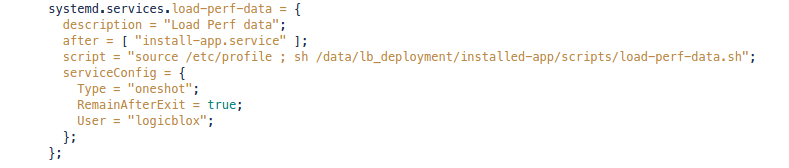
\includegraphics[width=14cm]{load-perf-data}
\caption{Load perf data nix expression}
\label{fig:load-perf-data}
\end{figure}

\begin{figure}[h]
  \centerline{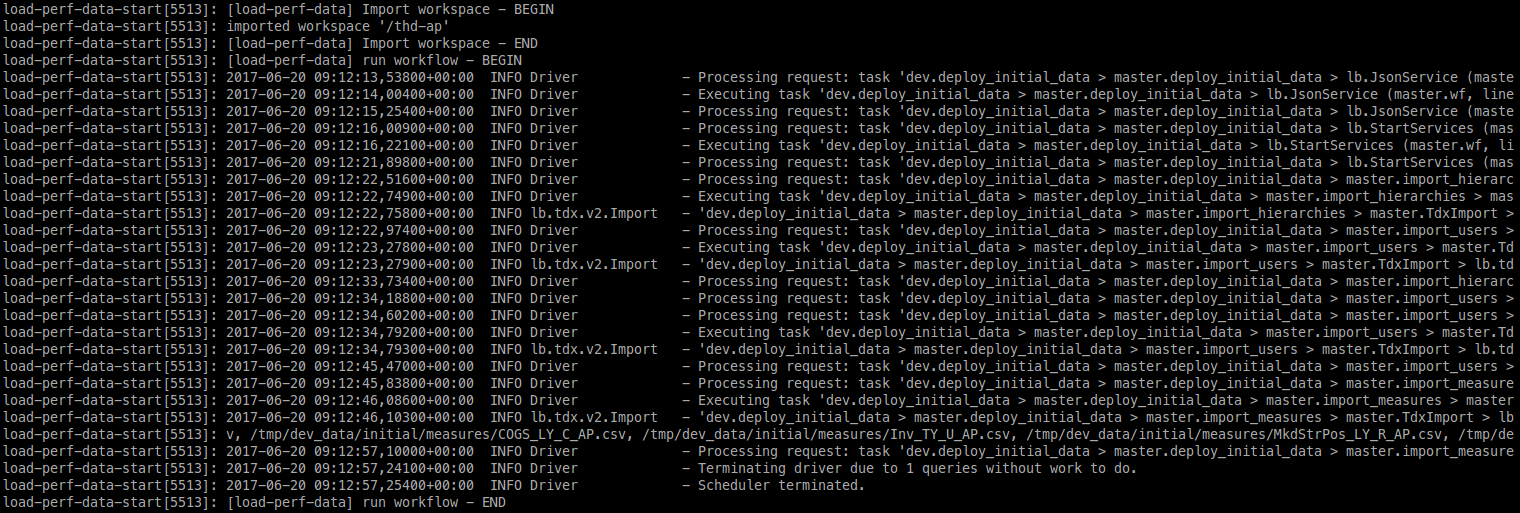
\includegraphics[width=14cm]{load-perf-data-log}}
\caption{load-perf-data log}
\label{fig:load-perf-data-log}
\end{figure}

\subsubsection{Running tests}
For running tests we use a generic script called \emph{run-perf}. This script will
define the instructions for running the tests, collect the logs, generate the
report and upload it to S3. The figure
\hyperref[fig:perf-runner-nix]{\ref{fig:perf-runner-nix}} shows the definition of
the systemd service \emph{perf-runner} responsible for running the script, it
will be launched as soon as the data is loaded with the \emph{load-perf-data}
service.
\begin{figure}[h]
  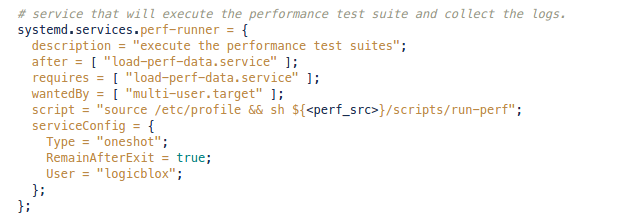
\includegraphics[width=14cm]{perf-runner-nix}
  \caption{perf-runner nix expression}
\label{fig:perf-runner-nix}
\end{figure}

\begin{figure}[h]
  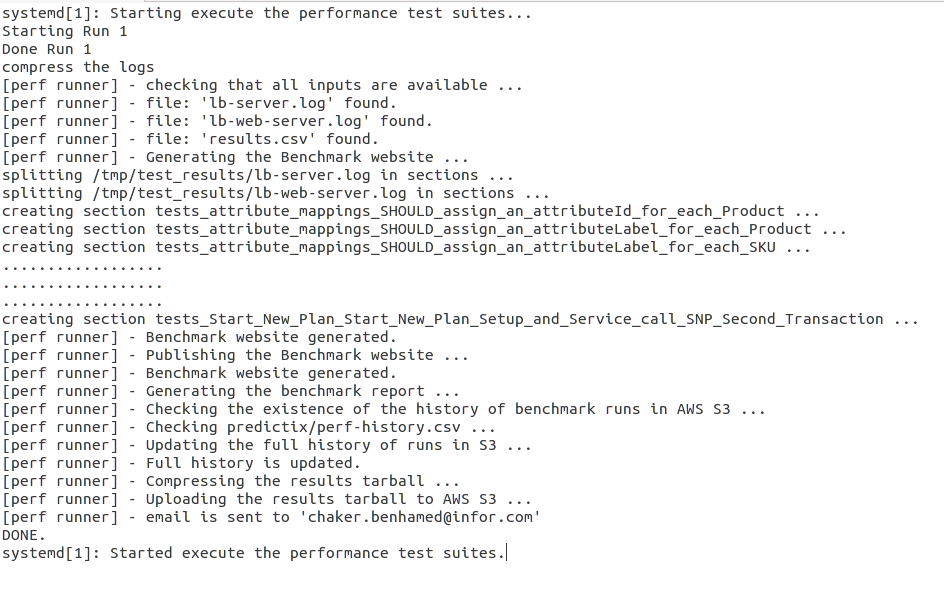
\includegraphics[width=14cm]{perf-runner-log}
  \caption{perf-runner log}
\label{fig:perf-runner-log}
\end{figure}
The figure \hyperref[fig:perf-runner-log]{\ref{fig:perf-runner-log}} shows a
trucated log of perf-runner service.

\section{Deployment}
Hydra is a Nix-based continuous build system that constantly checks out code
sources of software projects from version management systems such as Mercurial,
to build, test and release them. The build tasks are described using Nix
expressions. This allows a Hydra build task to specify all the dependencies
needed to build or test a project.

In fact, the code of our application is, currently and constantly pushed in a
repository in BitBucket, which is a web-based hosting service for projects that
use either the Mercurial or Git revision control systems, such as GitHub. In
order to have our application ready to be deployed, we added a file called
default.nix to our project, that actually defines our project’s nix-expressions.
Afterwards, we created a project under Hydra, that we called \emph{Benchmarks
  Dashboard}. Thus, the \emph{Benchmarks Dashboard} project on Hydra, will be
pulling our code from our BitBucket repository along with the default.nix file
in order to perform the automated build and unit-tests.

The following are some screen shots about our Hydra project build. The figure
\hyperref[fig:hydra_configuration]{\ref{fig:hydra_configuration}}
represents the configuration for our project. We can notice that the links to the
different project's dependencies are defined, such as our source code and the
nixpkgs repository which contains the definitions for all packages available through
the nix package manager.

\begin{figure}[h]
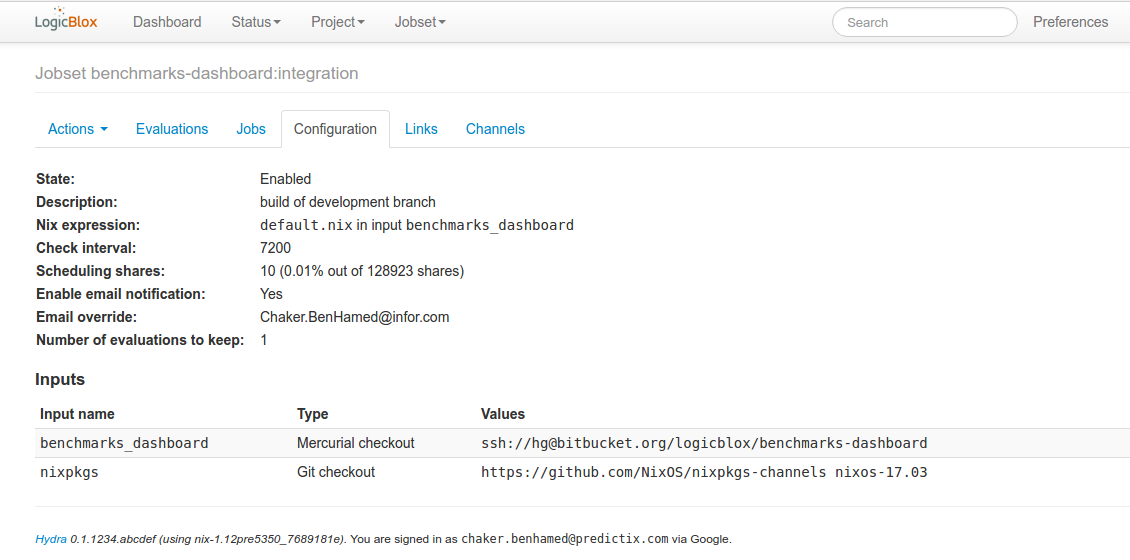
\includegraphics[width=17cm]{hydra_configuration}
\caption{Benchmarks Dashboard Hydra configuration screen}
\label{fig:hydra_configuration}
\end{figure}

The figure \hyperref[fig:hydra_eval]{\ref{fig:hydra_eval}} represents the Hydra
evaluation screen, where we can see the history if the build and whether there
are erros in the build or not.

\begin{figure}[h]
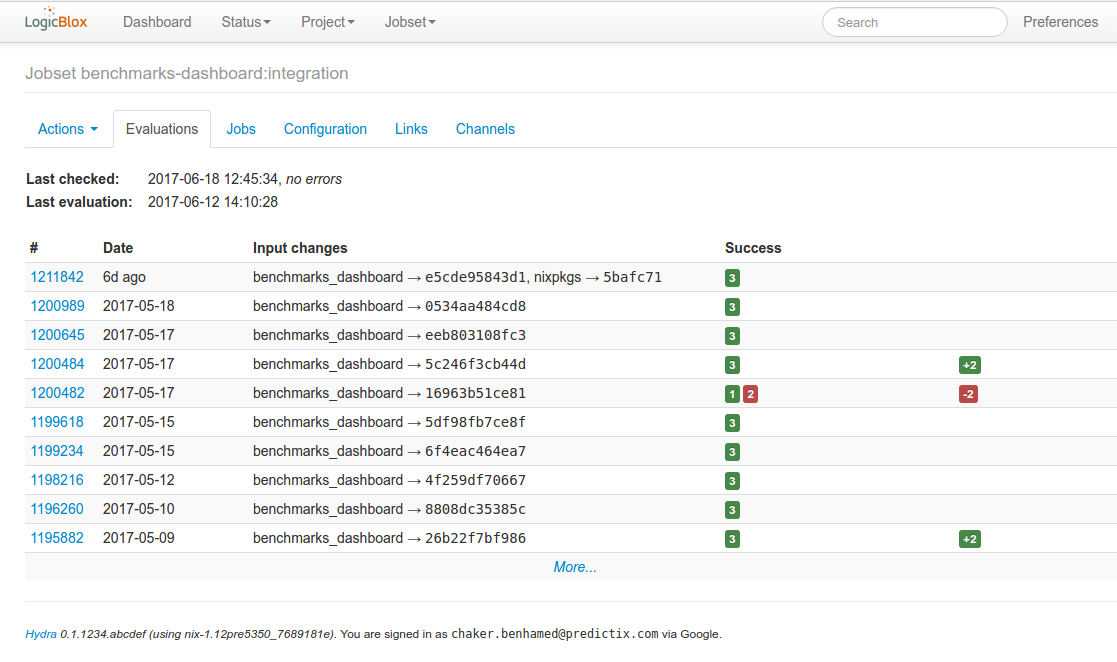
\includegraphics[width=17cm]{hydra_eval}
\caption{Benchmarks Dashboard Hydra configuration screen}
\label{fig:hydra_eval}
\end{figure}

In Hydra we can also run unit test and report various indicator about the
quality of the application. The figure
\hyperref[fig:coverage]{\ref{fig:coverage}} shows the covarge report of the test
of our application.

\begin{figure}[h]
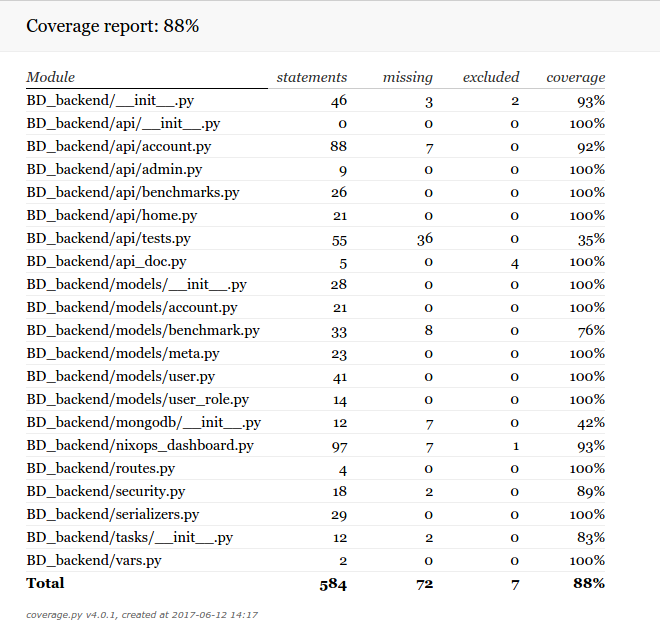
\includegraphics[width=17cm]{coverage}
\caption{Coverage report}
\label{fig:coverage}
\end{figure}

\clearpage
\section*{Conclusion}
TODO
